\chapter{Programowanie dynamiczne}

\makeatletter
\def\input@path{{chapter15/}}
\makeatother

\subchapter{Planowanie czynności na liniach montażowych}

\exercise %15.1-1
Poniższa rekurencyjna procedura wypisuje wszystkie stanowiska o~numerach od 1 do $j$ w~kolejności rosnącej, przy założeniu, że linia użyta na stanowisku $j$ ma numer $i$.
Do wywołania rekurencyjnego przekazywany jest numer wykorzystanej linii na stanowisku $j-1$ odczytany z~$l_i[j]$.
Imitowane jest dzięki temu zachowanie pętli z~oryginalnej procedury.
\begin{codebox}
\Procname{$\proc{Print-Stations-Increasing}(l,i,j)$}
\li	\If $j\ge1$
\li	\Then $\proc{Print-Stations-Increasing}(l,l_i[j],j-1)$
\li		wypisz ,,linia '' $i$ ,,{}, stanowisko '' $j$
	\End
\end{codebox}
Aby wypisać cały ciąg stanowisk, należy wywołać $\proc{Print-Stations-Increasing}(l,l^*\!,n)$.

\exercise %15.1-2
W~pierwszym kroku indukcyjnym wzór oczywiście zachodzi:
\[
	r_1(n) = r_2(n) = 1 = 2^{n-n}.
\]
Niech teraz $j=1$, 2, \dots, $n-1$ i~przyjmijmy, że $r_1(j+1)=r_2(j+1)=2^{n-(j+1)}$.
Stąd
\[
	r_1(j) = r_2(j) = r_1(j+1)+r_2(j+1) = 2^{n-(j+1)}+2^{n-(j+1)} = 2^{n-(j+1)+1} = 2^{n-j},
\]
a~więc wzór jest prawdziwy dla dowolnego $j$.

\exercise %15.1-3
Na podstawie wyniku poprzedniego zadania oraz wzoru (A.5), łączna liczba odwołań do wartości $f_i[j]$ wynosi:
\[
	\sum_{i=1}^2\sum_{j=1}^nr_i(j) = 2\sum_{j=1}^n2^{n-j} = 2\sum_{k=0}^{n-1}2^k = 2\cdot\frac{2^n-1}{2-1} = 2^{n+1}-2.
\]

\exercise %15.1-4
Możemy zrezygnować z~większości komórek tablic $f_i$.
Wystarczy zauważyć, że jedynymi wartościami z~tablic $f_i$ potrzebnymi do obliczenia $f_i[j]$ są $f_i[j-1]$.
Tablice $f_i$ nie są też wykorzystywane podczas wypisywania optymalnego rozwiązania w~procedurze \proc{Print-Stations}.
Dokładniej mówiąc, w~procedurze \proc{Fastest-Way} wystarczy zaalokować jedynie $f_1[1\twodots2]$ oraz $f_2[1\twodots2]$, czyli w~sumie 4 komórki.
Na pozycji $f_i[1]$ zapisane zostaną wartości dla poprzedniego stanowiska i~wykorzystane następnie do obliczenia wartości dla obecnego stanowiska, które zostaną zapamiętane w~$f_i[2]$.
Na początku każdej iteracji pętli \kw{for} $f_i[1]$ będzie nadpisywane przez $f_i[2]$.
Dzięki tej modyfikacji tablice $f_i$ i~$l_i$ będą zawierać łącznie $4+(2n-2)=2n+2$ pozycji.

\exercise %15.1-5
Przypisanie $l_1[j]\gets2$ wykonywane jest w~procedurze \proc{Fastest-Way} tylko w~linii 8 i~odbywa się jedynie wtedy, gdy warunek z~wiersza 4 jest fałszywy.
Podobnie, przypisanie $l_2[j]\gets1$ odbywa się jedynie wtedy, gdy warunek z~wiersza 9 jest fałszywy.
Oba te przypisania zostaną więc wykonane dla tego samego $j$, o~ile spełnione zostaną nierówności
\[
	f_1[j-1]+a_{1,j}>f_2[j-1]+t_{2,j-1}+a_{1,j} \quad\text{oraz}\quad f_2[j-1]+a_{2,j}>f_1[j-1]+t_{1,j-1}+a_{2,j}.
\]
Jednakże po dodaniu ich stronami i~zredukowaniu powtarzających się wyrazów, otrzymujemy $t_{1,j-1}+t_{2,j-1}<0$, co jest sprzeczne z~założeniem.

\subchapter{Mnożenie ciągu macierzy}

\exercise %15.2-1
Posługując się algorytmami \proc{Matrix-Chain-Order} i~\proc{Print-Optimal-Parens}, dostajemy, że dla ciągu macierzy $\langle A_1,\dots,A_6\rangle$ o~zadanych rozmiarach, optymalnym nawiasowaniem jest $((A_1A_2)((A_3A_4)(A_5A_6)))$.
Mnożąc macierze zgodnie z~tym nawiasowaniem, wykonamy 2010 mnożeń skalarnych.

\exercise %15.2-2
Nasz algorytm oprzemy na \proc{Print-Optimal-Parens}, ale zamiast wypisywać nawiasowanie, będziemy przekazywać macierze zwrócone przez wywołania rekurencyjne do procedury odpowiedzialnej za rzeczywiste ich pomnożenie.
\begin{codebox}
\Procname{$\proc{Matrix-Chain-Multiply}(A,s,i,j)$}
\li	\If $i=j$
\li		\Then \Return $A_i$
		\End
\li	\Return $\proc{Matrix-Multiply}($
\zi	\>\>\> $\proc{Matrix-Chain-Multiply}(A,s,i,s[i,j]),$
\zi	\>\>\> $\proc{Matrix-Chain-Multiply}(A,s,s[i,j]+1,j))$
\end{codebox}

\exercise %15.2-3
Udowodnimy przez indukcję, że $P(n)\ge2^{n-2}$ dla każdego $n\ge1$, co pozwoli nam wywnioskować, że $P(n)=\Omega(2^n)$.

W~przypadkach, gdy $n=1$, 2, 3, 4, nierówność jest spełniona:
\begin{align*}
	P(1) &= 1 \ge 2^{1-2}, \\
	P(2) &= P(1)P(1) = 1 \ge 2^{2-2}, \\
	P(3) &= P(1)P(2)+P(2)P(1) = 1+1 = 2 \ge 2^{3-2}, \\
	P(4) &= P(1)P(3)+P(2)P(2)+P(3)P(1) = 2+1+2 = 5 \ge 2^{4-2}.
\end{align*}
Niech teraz $n\ge5$.
Dla każdego $i=1$, \dots, $n-1$ przyjmiemy założenie indukcyjne $P(i)\ge2^{i-2}$.
Mamy wówczas:
\[
	P(n) = \sum_{k=1}^{n-1}P(k)P(n-k) \ge \sum_{k=1}^{n-1}2^{k-2}2^{n-k-2} = \sum_{k=1}^{n-1}2^{n-4} = \frac{n-1}{4}\cdot2^{n-2}.
\]
Gdy $n\ge5$, to $(n-1)/4\ge1$, dlatego otrzymujemy $P(n)\ge2^{n-2}$.

\exercise %15.2-4
W~celu obliczenia $m[i,j]$, w~każdej iteracji pętli \kw{for} w~wierszach 8\nbendash12 wykorzystywane są dwie inne wartości z~tej tablicy.
Łączna liczba odwołań do tablicy $m$ jest zatem dwukrotnie większa od sumarycznej liczby iteracji najbardziej wewnętrznej pętli.
Mamy więc:
\begin{align*}
	\sum_{i=1}^n\sum_{j=i}^nR(i,j) &= \sum_{l=2}^n\sum_{i=1}^{n-l+1}\sum_{k=i}^{i+l-2}2 \\
	&= \sum_{l=2}^n2(l-1)(n-l+1) \\
	&= \sum_{l=1}^{n-1}2l(n-l) \\
	&= 2n\sum_{l=1}^{n-1}l-2\sum_{l=1}^{n-1}l^2 \\
	&= 2n\cdot\frac{n(n-1)}{2}-2\cdot\frac{n(n-1)(2n-1)}{6} \\
	&= n^3-n^2-\frac{2n^3-3n^2+n}{3} \\
	&= \frac{n^3-n}{3}.
\end{align*}

\exercise %15.2-5
Obserwację udowodnimy przez indukcję po długości $n$ wyrażenia $\Phi$.
Jeśli $n=1$, to pojedynczy element wyrażenia $\Phi$ sam w~sobie ma ustalone pełne nawiasowanie -- występuje tu zatem 0 par nawiasów i~podstawa indukcji zachodzi.

Niech teraz $n\ge2$.
Załóżmy, że dla każdego wyrażenia o~$k<n$ elementach w~ich pełnym nawiasowaniu występuje dokładnie $k-1$ par nawiasów.
Rozważmy teraz dowolne pełne nawiasowanie wyrażenia $\Phi$ o~$n\ge2$ elementach.
Z~definicji mamy, że istnieje $k$ takie, że $1<k<n$ i~wyrażenie $\Phi$ stanowi iloczyn podwyrażenia o~$k$ elementach i~podwyrażenia o~$n-k$ elementach, oba o~ustalonych pełnych nawiasowaniach.
Założenie indukcyjne mówi, że pełne nawiasowania tych podwyrażeń mają, odpowiednio, $k-1$ i~$n-k-1$ par nawiasów.
Dodając do tych liczb dodatkową parę nawiasów, która obejmuje całe wyrażenie $\Phi$, mamy, że łącznie w~pełnym nawiasowaniu $\Phi$ występuje $(k-1)+(n-k-1)+1=n-1$ par nawiasów.

\subchapter{Podstawy programowania dynamicznego}

\exercise %15.3-1
Efektywniejszą metodą znajdowania optymalnego nawiasowania iloczynu ciągu macierzy jest wywołanie procedury \proc{Recursive-Matrix-Chain}.
Aby się o~tym przekonać, przyjrzyjmy się działaniu obu metod dla podciągu $A_iA_{i+1}\dots A_j$.

Procedura \proc{Recursive-Matrix-Chain} tworzy podziały tego podciągu na dwie części i~rekurencyjnie rozwiązuje powstałe podproblemy.
Dokładniej, dla każdego $k=i$, $i+1$, \dots, $j-1$ oddzielnie znajduje rozwiązanie dla podciągu $A_iA_{i+1}\dots A_k$ i~podciągu $A_{k+1}A_{k+2}\dots A_j$, a~następnie łączy te rozwiązania, aby otrzymać rozwiązanie dla $A_iA_{i+1}\dots A_j$.

Z~kolei w~trakcie generowania wszystkich poprawnych nawiasowań podciągu $A_iA_{i+1}\dots A_j$, dla każdego $k=i$, $i+1$, \dots, $j-1$ i~każdego poprawnego nawiasowania podciągu $A_iA_{i+1}\dots A_k$ zostanie rozważone każde poprawne nawiasowanie podciągu $A_{k+1}A_{k+2}\dots A_j$.
Oczywistym jest, że to podejście wymaga znacznie większej liczby operacji.
Jest tak dlatego, że nie wykorzystuje ono własności optymalnej podstruktury tego problemu.

\exercise %15.3-2
Sortowanie przez scalanie jest algorytmem realizującym podejście ,,dziel i~zwyciężaj'', w~którym początkowy problem dzielony jest na podproblemy rozwiązywane rekurencyjnie.
Powstające podproblemy nie powtarzają się pomiędzy wywołaniami rekurencyjnymi, co można zaobserwować na ilustracji drzewa rekursji tego algorytmu (rys.\ \ref{fig:15.3-2}).
W~drzewie tym każdy węzeł jest unikalny, inaczej niż w~przypadku drzewa rekursji algorytmu opartego na programowaniu dynamicznym, np.\ tego z~rys.\ 15.5 z Podręcznika.
Brak wspólnych podproblemów w~algorytmach opartych na metodzie ,,dziel i~zwyciężaj'' sprawia, że nie można ich przyspieszyć, stosując spamiętywanie.
\begin{figure}[!ht]
	\centering 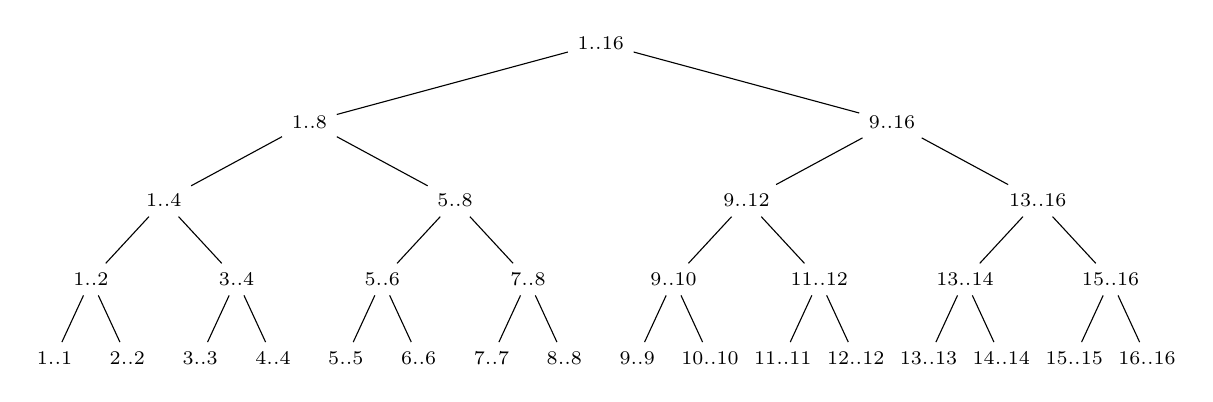
\begin{tikzpicture}[
	level/.append style = {level distance=10mm, sibling distance=148mm/2^#1},
	every node/.append style = {font=\scriptsize}
]

\node (root) {$1..16$}
	child {node {$1..8$}
		child {node {$1..4$}
			child {node {$1..2$}
				child {node {$1..1$}}
				child {node {$2..2$}}
			}
			child {node {$3..4$}
				child {node {$3..3$}}
				child {node {$4..4$}}
			}
		}
		child {node {$5..8$}
			child {node {$5..6$}
				child {node {$5..5$}}
				child {node {$6..6$}}
			}
			child {node {$7..8$}
				child {node {$7..7$}}
				child {node {$8..8$}}
			}
		}
	}
	child {node {$9..16$}
		child {node {$9..12$}
			child {node {$9..10$}
				child {node {$9..9$}}
				child {node {$10..10$}}
			}
			child {node {$11..12$}
				child {node {$11..11$}}
				child {node {$12..12$}}
			}
		}
		child {node {$13..16$}
			child {node {$13..14$}
				child {node {$13..13$}}
				child {node {$14..14$}}
			}
			child {node {$15..16$}
				child {node {$15..15$}}
				child {node {$16..16$}}
			}
		}
	};

\end{tikzpicture}

	\caption{Drzewo rekursji dla procedury \proc{Merge-Sort} działającej na tablicy z~16 elementami.
Każdy węzeł drzewa jest oznaczony zakresem $i\twodots j$ tablicy, na której działa procedura.} \label{fig:15.3-2}
\end{figure}

\exercise %15.3-3
Problem ten ma własność optymalnej podstruktury, o~czym można się przekonać podobnie, jak w~jego oryginalnej wersji.
W~tym wariancie optymalnym nawiasowaniem iloczynu macierzy będziemy nazywać takie nawiasowanie, które maksymalizuje liczbę mnożeń skalarnych.

Przypuśćmy, że w~optymalnym nawiasowaniu iloczynu $A_iA_{i+1}\dots A_j$ podział występuje między $A_k$ i~$A_{k+1}$.
Wówczas nawiasowanie podciągu $A_iA_{i+1}\dots A_k$, stanowiące część optymalnego nawiasowania iloczynu $A_iA_{i+1}\dots A_j$, musi być optymalne.
Gdyby bowiem istniał sposób ustawienia nawiasów w~ciągu $A_iA_{i+1}\dots A_k$ o~większym koszcie, to podmieniając nawiasowanie tego podciągu w~optymalnym nawiasowaniu $A_iA_{i+1}\dots A_j$, otrzymalibyśmy inne nawiasowanie dla $A_iA_{i+1}\dots A_j$, ale o~koszcie większym niż optymalny, co stanowi sprzeczność z~założeniem.
Podobne rozumowanie prowadzi do wniosku, że nawiasowanie podciągu $A_{k+1}A_{k+2}\dots A_j$ w~optymalnym nawiasowaniu $A_iA_{i+1}\dots A_j$ jest optymalne dla ciągu $A_{k+1}A_{k+2}\dots A_j$.

\exercise %15.3-4
W~problemie planowania czynności na liniach montażowych zarówno najszybszy sposób montażu do stanowiska $S_{1,j}$, jak i~najszybszy sposób montażu do stanowiska $S_{2,j}$, polega na optymalnych czasach montażu do stanowisk $S_{1,j-1}$ i~$S_{2,j-1}$.
Innymi słowy, wartości $f_1[j-1]$ oraz $f_2[j-1]$ wykorzystywane są do obliczenia zarówno $f_1[j]$, jak i~$f_2[j]$.

\exercise %15.3-5
Jednym z~kontrprzykładów jest ciąg macierzy $\langle A_1,A_2,A_3\rangle$ o~rozmiarach stanowiących ciąg $\langle1,2,5,4\rangle$.
Liczbą mnożeń skalarnych wykonywanych podczas mnożenia $A_1$ przez $(A_2A_3)$ jest $1\cdot2\cdot4=8$, a~podczas mnożenia $(A_1A_2)$ przez $A_3$ -- $1\cdot5\cdot4=20$.
W~podejściu zachłannym podział iloczynu $A_1A_2A_3$ zostanie zatem wyznaczony między macierzą $A_1$ a~$A_2$ i~wynikowym nawiasowaniem będzie $(A_1(A_2A_3))$ z~kosztem $2\cdot5\cdot4+1\cdot2\cdot4=48$ mnożeń skalarnych.
Rozwiązaniem optymalnym jest jednak nawiasowanie $((A_1A_2)A_3)$ o~koszcie $1\cdot2\cdot5+1\cdot5\cdot4=30$.

\subchapter{Najdłuższy wspólny podciąg}

\exercise %15.4-1
Dla zadanych ciągów NWP wyznaczonym przez procedury \proc{LCS-Length} i~\proc{Print-LCS} jest $\langle1,0,0,1,1,0\rangle$.
Poza nim istnieje jeszcze 7 innych NWP tych ciągów:
\begin{gather*}
	\langle0,0,1,0,1,0\rangle, \\
	\langle0,0,1,0,1,1\rangle, \\
	\langle0,0,1,1,0,1\rangle, \\
	\langle0,1,0,1,0,1\rangle, \\
	\langle1,0,1,0,1,0\rangle, \\
	\langle1,0,1,0,1,1\rangle, \\
	\langle1,0,1,1,0,1\rangle.
\end{gather*}

\exercise %15.4-2
Poniższy pseudokod stanowi implementację zmodyfikowanej wersji procedury \proc{Print-LCS}, która wypisuje NWP ciągów $X$ i~$Y$ bez korzystania z~tablicy $b$.
Zamiast tego przyjmuje tablicę $c$ oraz dodatkowo ciąg $Y$.
Pierwsze wywołanie procedury powinno być następujące: $\proc{Print-LCS}'(c,X,Y,\attrib{X}{length},\attrib{Y}{length})$.
\begin{codebox}
\Procname{$\proc{Print-LCS}'(c,X,Y,i,j)$}
\li	\If $i=0$ lub $j=0$
\li		\Then \Return
		\End
\li	\If $x_i=y_j$
\li		\Then $\proc{Print-LCS}'(c,X,Y,i-1,j-1)$
\li			wypisz $x_i$
\li		\ElseIf $c[i,j]=c[i-1,j]$
\li			\Then $\proc{Print-LCS}'(c,X,Y,i-1,j)$
\li		\ElseNoIf $\proc{Print-LCS}'(c,X,Y,i,j-1)$
		\End
\end{codebox}

Wprowadzone modyfikacje w~tej procedurze nie wpływają na czas jej działania w~porównaniu z~oryginalną \proc{Print-LCS}.

\exercise %15.4-3
W~naszej implementacji będziemy obliczać kolejne wartości rekurencyjnie bezpośrednio ze wzoru (15.14), ale z~wykorzystaniem tablicy $c[0\twodots m,0\twodots n]$ i~mechanizmu spamiętywania.
Aby zaznaczyć, że dane pole tablicy $c$ nie zostało jeszcze obliczone, użyjemy specjalnej wartości $\infty$.
Pierwsza z~procedur inicjalizuje tablicę $c$, po czym wywołuje właściwy algorytm odpowiedzialny za obliczenie wartości $c[m,n]$.
\begin{codebox}
\Procname{$\proc{Memoized-LCS-Length}(X,Y)$}
\li	$m\gets\attrib{X}{length}$
\li	$n\gets\attrib{Y}{length}$
\li	\For $i\gets0$ \To $m$
\li		\Do \For $j\gets0$ \To $n$
\li				\Do $c[i,j]\gets\infty$ \label{li:memoized-lcs-length-init}
				\End
		\End
\li	\Return $\proc{Lookup-LCS}(c,X,Y,m,n)$
\end{codebox}
\begin{codebox}
\Procname{$\proc{Lookup-LCS}(c,X,Y,i,j)$}
\li	\If $c[i,j]<\infty$
\li		\Then \Return $c[i,j]$
		\End
\li	\If $i=0$ lub $j=0$
\li		\Then $c[i,j]\gets0$
\li		\ElseIf $x_i=y_j$
\li			\Then $c[i,j]\gets\proc{Lookup-LCS}(c,X,Y,i-1,j-1)+1$
\li		\ElseNoIf $c[i,j]\gets\max(\proc{Lookup-LCS}(c,X,Y,i,j-1),\proc{Lookup-LCS}(c,X,Y,i-1,j))$
		\End
\li	\Return $c[i,j]$
\end{codebox}

Każde z~$(m+1)(n+1)$ pól tablicy $c$ zostaje zainicjalizowane w~wierszu \ref{li:memoized-lcs-length-init} pierwszej procedury, a~następnie zmodyfikowane przez jedno wywołanie algorytmu \proc{Lookup-LCS}.
Wywołania \proc{Lookup-LCS} możemy podzielić na dwa typy:
\begin{enumerate}[(i)]
	\item wywołania, w~których $c[i,j]=\infty$, oraz
	\item wywołania, w~których $c[i,j]<\infty$.
\end{enumerate}
Wywołań pierwszego typu jest dokładnie $\Theta(mn)$, jedno na każde pole tablicy $c$, a~każde z~nich jest wykonywane w~czasie $\Theta(1)$ plus czas spędzany na obliczenia rekurencyjne.
Do każdego wywołania drugiego typu może doprowadzić rekursja podczas wywołania pierwszego typu.
Kiedy w~danym wywołaniu \proc{Lookup-LCS} pojawiają się wywołania rekurencyjne, jest ich $\Theta(1)$, dlatego łącznie wywołań drugiego typu jest $\Theta(mn)$, z~których każde zabiera czas $\Theta(1)$.
Stąd całkowity czas wykonania procedury \proc{Memoized-LCS-Length} wynosi $\Theta(mn)$.

\exercise %15.4-4
Zauważmy, że do obliczenia $c[i,j]$ w~procedurze \proc{LCS-Length} wykorzystywane są wartości $c[i-1,j]$, $c[i,j-1]$ oraz $c[i-1,j-1]$.
Możemy więc utrzymywać tylko 2 wiersze tablicy $c$ -- wiersz aktualnie obliczany oraz wiersz bezpośrednio go poprzedzający.
Po każdej iteracji poprzedni wiersz będzie nadpisywany wartościami z~bieżącego wiersza, aby przygotować tablicę do kolejnej iteracji.
Aby tablica $c$ była rozmiaru $2\cdot\min(m,n)$, przed jej utworzeniem należy jeszcze sprawdzić, czy $n\le m$.
Jeśli nie, to wystarczy uruchomić procedurę z~ciągami $X$ i~$Y$ zamienionymi miejscami.

Można jednak jeszcze bardziej ograniczyć zapotrzebowanie procedury na pamięć.
Załóżmy, że $n<m$.
Dwuwymiarowa tablica $c$ może zostać zamieniona na jednowymiarową tablicę $C[0\twodots n]$ przechowującą wartości z~tablicy $c$ z~wiersza $i-1$ oraz nadpisujące je wartości z~wiersza $i$.
Dokładniej, w~momencie obliczania $c[i,j]$ fragment $C[0\twodots j-1]$ zawiera kolejne wartości $c[i,0\twodots j-1]$, a~fragment $C[j\twodots n]$ -- kolejne wartości $c[i-1,j\twodots n]$.
Jeśli w~osobnej zmiennej $p$ zapamiętamy $c[i-1,j-1]$, czyli wartość $C[j-1]$ zanim została zaktualizowana w~poprzedniej iteracji, to będziemy dysponować wszystkimi danymi potrzebnymi do obliczenia $C[j]$.
Jeśli $x_i=y_j$, to $C[j]$ ustawione zostanie na $p+1$, co odpowiada wierszowi 10 z~oryginalnej procedury \proc{LCS-Length}.
W~przeciwnym przypadku do $C[j]$ wpisane zostanie $\max(C[j],C[j-1])$, co odpowiada wierszom 12\nbendash16.
Ostatnim krokiem w~bieżącej iteracji pętli jest aktualizacja zmiennej $p$ na wartość znajdującą się w~$C[j]$ przed modyfikacją tej komórki.
Dzięki tak wprowadzonym zmianom w~procedurze wykorzystujemy $\min(m,n)+\Theta(1)$ pamięci.

\exercise %15.4-5
W~\textbf{problemie najdłuższego niemalejącego podciągu} (w~skrócie: problemu NNP) dla danego ciągu $X=\langle x_1,x_2,\dots,x_n\rangle$ szukany jest jego podciąg o~największej możliwej długości, którego wyrazy ustawione są w~porządku niemalejącym.
Niech $X'$ będzie ciągiem powstałym z~$X$ po uporządkowaniu jego elementów niemalejąco.
Udowodnimy, że rozwiązaniem problemu NNP dla $X$ jest NWP ciągów $X$ i~$X'$.

\begin{proof}
Niech $W$ będzie NWP ciągów $X$ i~$X'$.
Jest on oczywiście podciągiem $X$ i~jest niemalejący, bo jest podciągiem ciągu niemalejącego $X'$.
Załóżmy nie wprost, że NNP ciągu $X$ jest ciąg $W'$ dłuższy od $W$.
Ale z~definicji NNP $W'$ jest też podciągiem $X$ i~jest niemalejący o~wyrazach z~$X$, czyli musi stanowić też podciąg $X'$.
Stąd $W'$ stanowi wspólny podciąg ciągów $X$ i~$X'$, co jest sprzeczne z~definicją $W'$.
\end{proof}

Algorytm znajdujący NNP ciągu $X$ może więc posortować wyrazy jego kopii, otrzymując $X'$, wywołać $\proc{LCS-Length}(X,X')$, a~na końcu wypisać znaleziony NNP procedurą \proc{Print-LCS}.
Czas działania tego algorytmu wynosi $O(n^2)$.

\exercise %15.4-6
Dla ciągu wejściowego $X=\langle x_1,x_2,\dots,x_n\rangle$, w~którym najdłuższy niemalejący podciąg (w~skrócie: NNP) ma długość $m$, niech $Z=\langle z_1,z_2,\dots,z_m\rangle$ będzie ciągiem takim, że $z_i$ jest najmniejszym elementem w~$X$ kończącym pewien podciąg niemalejący ciągu $X$ o~długości $i$.
Kluczowa jest własność ciągu $Z$ podana we wskazówce, czyli to, że jest on niemalejący.
Podamy krótki dowód tego faktu.
Załóżmy nie wprost, że istnieją indeksy $i$, $j$, takie, że $i<j$ oraz $z_i>z_j$.
Oznacza to, że najmniejszy element ciągu $X$ będący ostatnim elementem niemalejącego podciągu $X$ o~długości $i$ jest większy niż najmniejszy element ciągu $X$ kończący pewien niemalejący podciąg $X$ o~długości $j$.
Moglibyśmy jednak usunąć $j-i$ elementów z~podciągu o~długości $j$ zakończonego na $z_j$, otrzymując niemalejący podciąg ciągu $X$ o~długości $i$, w~którym ostatni element jest mniejszy niż $z_i$.
Sprzeczność.

Zamiast zapamiętywania ciągu $Z$, w~algorytmie będziemy korzystać z~tablicy $a[0\twodots n]$, w~której na $j$\nbhyphen tej pozycji, gdzie $j=1$, 2, \dots, $m$, będziemy przechowywać indeks $i$, taki że $z_j=x_i$.
Dla pozycji $j=0$ oraz $j=m+1$, $m+2$, \dots, $n$, przyjmiemy $a[j]=0$.
Przechowywanie indeksów elementów pozwoli nam na zbudowanie tablicy $b$, dzięki której będzie można odtworzyć znaleziony NNP\@.

Załóżmy, że w~trakcie przeglądania ciągu $X$ od lewej do prawej, aktualnie przetwarzanym elementem jest $x_i$, a~w~zmiennej $m$ przechowywana jest długość najdłuższego niemalejącego podciągu fragmentu $\langle x_1$, \dots, $x_{i-1}\rangle$.
Niech $k$ będzie takim indeksem w~tablicy $a$, że $x_{a[j]}\le x_i$ dla każdego $j=1$, 2, \dots, $k-1$, oraz $x_{a[j]}>x_i$ dla każdego $j=k$, $k+1$, \dots, $m$.
Element $x_i$ stanowi zatem najmniejszy napotkany do tej pory element kończący pewien niemalejący podciąg ciągu $X$ o~długości $k$ -- na pozycję $a[k]$ można więc wpisać $i$.
Dzięki uporządkowaniu elementów ciągu $X$ o~indeksach z~tablicy $a$, liczbę $k$ dla każdego elementu $x_i$ jesteśmy w~stanie wyznaczać w~czasie logarytmicznym, stosując wyszukiwanie binarne.

\begin{codebox}
\Procname{$\proc{LMIS-Length}(X)$}
\li	$n\gets\attrib{X}{length}$
\li	\For $i\gets0$ \To $n$ \label{li:lmis-length-a-init-begin}
\li		\Do $a[i]\gets0$
		\End \label{li:lmis-length-a-init-end}
\li	$m\gets0$
\li	\For $i\gets1$ \To $n$ \label{li:lmis-length-for-begin}
\li		\Do $k\gets1$ \label{li:lmis-length-binary-search-begin}
\li			$l\gets m$
\li			\While $k\le l$
\li				\Do $j\gets\lfloor(k+l)/2\rfloor$
\li					\If $x_{a[j]}\le x_i$
\li						\Then $k\gets j+1$
\li						\Else $l\gets j-1$
						\End
				\End \label{li:lmis-length-binary-search-end}
\li			$a[k]\gets i$
\li			$b[i]\gets a[k-1]$
\li			\If $k>m$
\li				\Then $m\gets k$
				\End
		\End \label{li:lmis-length-for-end}
\li	\Return $m$, $b$ i~$a[m]$
\end{codebox}
Powyżej zaprezentowany algorytm realizuje opisane podejście.
W~wierszach \ref{li:lmis-length-a-init-begin}\nbendash\ref{li:lmis-length-a-init-end} tablica $a$ inicjalizowana jest zerami, aby zaznaczyć, że żaden z~elementów ciągu $Z$ nie jest jeszcze znany.
Elementy ciągu $X$ przeglądane są następnie od lewej do prawej.
W~wierszach \ref{li:lmis-length-binary-search-begin}\nbendash\ref{li:lmis-length-binary-search-end} dla elementu $x_i$ odbywa się wyszukiwanie odpowiedniego indeksu tablicy $a$, gdzie należy umieścić $i$, aby zachować uporządkowanie elementów ciągu $X$ indukowane przez fragment $a[1\twodots m]$.
Po aktualizacji odpowiedniej komórki tablicy $a$, do $b[i]$ wpisywany jest indeks poprzedniego elementu w~ciągu $Z$ (lub 0, jeśli element $x_i$ rozpoczyna nowy podciąg niemalejący), a~następnie aktualizowana jest wartość zmiennej $m$.
Procedura zwraca informacje służące do odtworzenia znalezionego NNP\@.
Można go otrzymać (w~odwrotnej kolejności) przez wypisanie $x_{a[m]}$, a~następnie $x_{b[a[m]]}$, $x_{b[b[a[m]]}$ itd., dopóki indeks nie jest zerem.
Następująca rekurencyjna procedura pozwala wypisać NNP we właściwej kolejności:
\begin{codebox}
\Procname{$\proc{Print-LMIS}(b,X,i)$}
\li	\If $b[i]>0$
\li		\Then $\proc{Print-LMIS}(b,X,b[i])$
		\End
\li	wypisz $x_i$
\end{codebox}
Dysponując tablicą $b$ i~wartością $a[m]$ wyznaczonymi dla danego ciągu $X$, możemy wypisać jego NNP, wywołując $\proc{Print-LMIS}(b,X,a[m])$.

Każda iteracja pętli \kw{for} w~liniach \ref{li:lmis-length-for-begin}\nbendash\ref{li:lmis-length-for-end} algorytmu \proc{LMIS-Length} przeprowadza wyszukiwanie binarne w~podtablicy zawierającej co najwyżej $n$ elementów.
Poza pętlą inicjalizującą tablicę $a$ pozostałe operacje wykonywane w~procedurze zajmują czas co najwyżej stały.
Stąd algorytm działa w~czasie $O(n\lg n)$.

\subchapter{Optymalne drzewa wyszukiwań binarnych}

\exercise %15.5-1
Algorytm podzielimy na 3 procedury.
Pierwsza z~nich ma za zadanie wypisać korzeń optymalnego drzewa BST oraz wywołać drugą, rekurencyjną procedurę wypisującą strukturę tego drzewa.
W~tym celu dla danej tablicy \id{root} oraz pozycji $i\le j$ konstruowane jest poddrzewo o~korzeniu, którego indeks znajduje się w~$\id{root}[i,j]$.
Konstrukcja ta polega na wypisaniu jego lewego poddrzewa, a~następnie na wypisaniu jego prawego poddrzewa.
Trzecia procedura służy nam do pozyskiwania nazw węzłów na podstawie wartości w~tablicy \id{root} oraz pozycji w~niej.
\begin{codebox}
\Procname{$\proc{Construct-Optimal-BST}(\id{root})$}
\li	$n\gets\attribii{root}{length}$
\li	wypisz $\proc{Optimal-BST-Node}(\id{root},i,n)$ ,, jest korzeniem''
\li	$\proc{Construct-Optimal-BST-Subtree}(\id{root},1,n)$
\end{codebox}
\begin{codebox}
\Procname{$\proc{Construct-Optimal-BST-Subtree}(\id{root},i,j)$}
\li	\If $i\le j$
\li		\Then wypisz $\proc{Optimal-BST-Node}(\id{root},i,\id{root}[i,j]-1)$ ,, jest lewym synem $k$''$\!{}_{\id{root}[i,j]}$
\li			$\proc{Construct-Optimal-BST-Subtree}(\id{root},i,\id{root}[i,j]-1)$
\li			wypisz $\proc{Optimal-BST-Node}(\id{root},\id{root}[i,j]+1,j)$ ,, jest prawym synem $k$''$\!{}_{\id{root}[i,j]}$
\li			$\proc{Construct-Optimal-BST-Subtree}(\id{root},\id{root}[i,j]+1,j)$
		\End
\end{codebox}
\begin{codebox}
\Procname{$\proc{Optimal-BST-Node}(\id{root},i,j)$}
\li	\If $i\le j$
\li		\Then \Return ,,$k$''$\!{}_{\id{root}[i,j]}$
\li		\Else \Return ,,$d$''$\!{}_j$
		\End
\end{codebox}

\exercise %15.5-2
Algorytm \proc{Optimal-BST} wywołany dla zadanych prawdopodobieństw zwraca optymalne drzewo BST przedstawione na rys.\ \ref{fig:15.5-2}.
Tabela \ref{tab:15.5-2} ilustruje, podobnie jak w~Podręczniku, oczekiwany koszt wyszukiwania w~tym drzewie oraz wkład, jaki wprowadza w~ten koszt każdy węzeł.
\begin{figure}[!ht]
	\centering \begin{tikzpicture}[
	level/.append style = {level distance=7mm, sibling distance=120mm/2^#1},
	every node/.style = {tree node}
]

\newcommand\leafnode[1]{%
	node[align=center, inner sep=1pt, minimum size=5mm, rectangle, rounded corners=3pt, draw] {#1}
}

\node (root) {$k_5$}
	child {node {$k_2$}
		child {node {$k_1$}
			child[shorten >=-1pt] {\leafnode {$d_0$}}
			child[shorten >=-1pt] {\leafnode {$d_1$}}
		}
		child {node {$k_3$}
			child[shorten >=-1pt] {\leafnode {$d_2$}}
			child {node {$k_4$}
				child {\leafnode {$d_3$}}
				child {\leafnode {$d_4$}}
			}
		}
	}
	child {node {$k_7$}
		child {node {$k_6$}
			child[shorten >=-1pt] {\leafnode {$d_5$}}
			child [shorten >=-1pt]{\leafnode {$d_6$}}
		}
		child {\leafnode {$d_7$}}
	};

\end{tikzpicture}

	\caption{Optymalne drzewo BST dla zadanego ciągu prawdopodobieństw.} \label{fig:15.5-2}
\end{figure}
\begin{table}[!ht]
	\centering
		\begin{tabular}{cccc}
			węzeł & głębokość & prawdopodobieństwo & wkład \\ \hline
			$k_1$ & 2 & 0{,}04 & 0{,}12 \\
			$k_2$ & 1 & 0{,}06 & 0{,}12 \\
			$k_3$ & 2 & 0{,}08 & 0{,}24 \\
			$k_4$ & 3 & 0{,}02 & 0{,}08 \\
			$k_5$ & 0 & 0{,}10 & 0{,}10 \\
			$k_6$ & 2 & 0{,}12 & 0{,}36 \\
			$k_7$ & 1 & 0{,}14 & 0{,}28 \\
			$d_0$ & 3 & 0{,}06 & 0{,}24 \\
			$d_1$ & 3 & 0{,}06 & 0{,}24 \\
			$d_2$ & 3 & 0{,}06 & 0{,}24 \\
			$d_3$ & 4 & 0{,}06 & 0{,}30 \\
			$d_4$ & 4 & 0{,}05 & 0{,}25 \\
			$d_5$ & 3 & 0{,}05 & 0{,}20 \\
			$d_6$ & 3 & 0{,}05 & 0{,}20 \\
			$d_7$ & 2 & 0{,}05 & 0{,}15 \\ \hline
			Razem & & & 3{,}12
		\end{tabular} \caption{Zestawienie kosztów wprowadzanych przez poszczególne węzły w~optymalnym drzewie BST dla podanych prawdopodobieństw.} \label{tab:15.5-2}
\end{table}

\exercise %15.5-3
Obliczanie wartości $w(i,j)$ bezpośrednio ze wzoru (15.17) wymaga wykonania $\Theta(j-i)$ dodawań.
Zauważmy, że pętla \kw{for} w~wierszach 9\nbendash13 wykonuje także $\Theta(j-i)$ iteracji, a~każda z~nich wymaga czasu stałego.
A~zatem modyfikacja ta nie wpłynie na asymptotyczny czas działania algorytmu, tylko co najwyżej na zwiększenie stałego czynnika ukrytego w~notacji $\Theta$.

\exercise %15.5-4
Wykorzystamy podaną obserwację i~w~najbardziej wewnętrznej pętli w~procedurze \proc{Optimal-BST}, zamiast iterować zmienną $r$ od $i$ do $j$, będziemy przebiegać wszystkie wartości od $\id{root}[i,j-1]$ do $\id{root}[i+1,j]$.
Aby jednak skorzystać z~tego usprawnienia, musimy upewnić się, że $i<j$.
Warunek ten zachodzi, gdy $l>1$, zatem w~pętli \kw{for} w~wierszach 4\nbendash13 zmienna $l$ będzie przyjmować wartości od 2 do $n$, natomiast działania wykonywane, gdy $l=1$, będziemy imitować następującym fragmentem, który wstawimy tuż przed tę pętlę:
\begin{codebox}
\zi	\For $i\gets1$ \To $n$
\zi		\Do $w[i,i]\gets w[i,i-1]+p_i+q_i$
\zi			$e[i,i]\gets e[i,i-1]+e[i+1,i]+w[i,i]$
\zi			$\id{root}[i,i]\gets i$
		\End
\end{codebox}

Pokażemy, że tablice $e$ i~\id{root} zostaną wypełnione w~czasie $\Theta(n^2)$.
Pętla w~wierszach 1\nbendash3 wraz z~tą stanowiącą nowy fragment wykonują w~sumie $2n+1$ iteracji.
Dla każdego $2\le l\le n$ pętla \kw{for} w~wierszach 9\nbendash13 wykona łącznie $S(n,l)=\sum_{i=1}^{n-l+1}(\id{root}[i+1,j]-\id{root}[i,j-1]+1)$ iteracji.
Po podstawieniu $j=i+l-1$ i~skorzystaniu z~własności sumy teleskopowej otrzymujemy:
\begin{align*}
	S(n,l) &= \sum_{i=1}^{n-l+1}(\id{root}[i+1,j]-\id{root}[i,j-1]+1) \\
	&= \sum_{i=1}^{n-l+1}(\id{root}[i+1,i+l-1]-\id{root}[i,i+l-2])+\sum_{i=1}^{n-l+1}1 \\
	&= \id{root}[n-l+2,n]-\id{root}[1,l-1]+n-l+1.
\end{align*}
Największą możliwą wartością różnicy $\id{root}[n-l+2,n]-\id{root}[1,l-1]$ jest $n-1$, skąd mamy $S(n,l)\le n-1+n-l+1\le2n-2$.
Sumaryczna liczba iteracji najbardziej wewnętrznej pętli wynosi więc $\sum_{l=2}^nS(n,l)\le2(n-1)^2=O(n^2)$.
Obliczana jest każda z~$n(n+1)/2$ z~komórek tablic $e$ i~\id{root}, dlatego dolnym ograniczeniem na czas potrzebny do ich wypełnienia jest oczywiście $\Omega(n^2)$.
Stąd czasem działania algorytmu jest $\Theta(n^2)$.


\problems

\problem{Bitoniczny problem komiwojażera} %15-1
Podążając za wskazówką z~treści problemu, będziemy przeglądać punkty wejściowe od lewej do prawej, po uprzednim posortowaniu ich po współrzędnych $x$.
Tak uporządkowane punkty oznaczymy przez $p_1$, $p_2$, \dots, $p_n$, a~więc $p_1$ jest punktem wysuniętym najbardziej na lewo, a~$p_n$ punktem wysuniętym najbardziej na prawo.

Dla $1\le i\le j\le n$ rozważmy zbiory $B_{i,j}$ ścieżek zawierających każdy punkt $p_1$, $p_2$, \dots, $p_j$ dokładnie raz, z~wyjątkiem przypadku $i=j$, w~którym $p_j$ występuje dokładnie 2 razy, i~mających postać $\langle p_i,\dots,p_1,\dots,p_j\rangle$, przy czym podścieżka $\langle p_i,\dots,p_1\rangle$ (złożona z~tylko jednego punktu, gdy $i=1$) biegnie po punktach o~malejących indeksach, a~podścieżka $\langle p_1,\dots,p_j\rangle$ (złożona z~tylko jednego punktu, gdy $j=1$) -- po punktach o~rosnących indeksach.
Przez $|pp'|$ oznaczymy odległość euklidesową między punktami $p$ i~$p'$, a~przez $b[i,j]$ -- długość mierzoną odległością euklidesową najkrótszej ścieżki ze zbioru $B_{i,j}$.
Zauważmy, że zbiory $B_{j,j}$ składają się ze ścieżek bitonicznych między punktami $p_1$, $p_2$, \dots, $p_j$.
Rozwiązanie problemu stanowi więc wartość $b[n,n]$.

Niech $\beta_{i,j}$ będzie najkrótszą ścieżką w~$B_{i,j}$.
Oczywiście $b[1,1]=0$, przyjmijmy więc, że $j>1$.
Gdy $i=1$ lub $i<j-1$, bezpośrednio przed $p_j$ na $\beta_{i,j}$ znajduje się punkt $p_{j-1}$.
Podścieżka $\langle p_i,\dots,p_{j-1}\rangle$ musi być najkrótszą ścieżką z~$B_{i,j-1}$; inaczej moglibyśmy ją ,,wyciąć'' i~,,wkleić'' w~jej miejsce podścieżkę z~tego zbioru o~mniejszej długości, uzyskując ścieżkę krótszą niż $\beta_{i,j}$.
Stąd długość $b[i,j]$ ścieżki $\beta_{i,j}$ wynosi $b[i,j-1]+|p_{j-1}p_j|$.
Jeśli z~kolei $i>1$ oraz zachodzi $i=j-1$ lub $i=j$, to punkt $p_j$ jest bezpośrednio poprzedzony pewnym punktem $p_k$, gdzie $k<i$.
Tutaj także ma miejsce optymalna podstruktura -- podścieżka $\langle p_i,\dots,p_k\rangle$ jest odwróconą najkrótszą ścieżką z~$B_{k,i}$, o~czym można się przekonać, stosując metodę ,,wytnij i~wklej''.
W~tym przypadku ścieżka $\beta_{i,j}$ ma długość $b[i,j]=\min_{1\le k<i}(b[k,i]+|p_kp_j|)$.
Na podstawie tej analizy dostajemy następującą zależność rekurencyjną:
\[
	b[i,j] = \begin{cases}
		0, & \text{jeśli $i=j=1$}, \\
		b[i,j-1]+|p_{j-1}p_j|, & \text{jeśli $i=1<j$ lub $i<j-1$}, \\
		\displaystyle\min_{1\le k<i}(b[k,i]+|p_kp_j|), & \text{w~pozostałych przypadkach}.
	\end{cases}
\]

Aby zrekonstruować rozwiązanie, dla każdych $1\le i<j\le n$ obliczymy $r[i,j]$, czyli indeks punktu bezpośrednio poprzedzającego $p_j$ na ścieżce $\beta_{i,j}$.
Poniższy pseudokod wyznacza wartości w~tablicach $b$ i~$r$, wykorzystując programowanie dynamiczne.
\begin{codebox}
\Procname{$\proc{Bitonic-TSP}(p)$}
\li	$n\gets\attrib{p}{length}$
\li	posortuj ciąg punktów wejściowych $p$ rosnąco względem ich współrzędnych $x$ \label{li:bitonic-tsp-sorting}
\li	$b[1,1]\gets0$
\li	\For $j\gets2$ \To $n$
\li		\Do \For $i\gets1$ \To $j$
\li				\Do \If $i=1$ lub $i<j-1$
\li						\Then $b[i,j]\gets b[i,j-1]+|p_{j-1}p_j|$
\li							$r[i,j]\gets j-1$
\li						\Else $b[i,j]\gets\infty$ \label{li:bitonic-tsp-min-begin}
\li							\For $k\gets1$ \To $i-1$
\li								\Do $q\gets b[k,i]+|p_kp_j|$
\li									\If $q<b[i,j]$
\li										\Then $b[i,j]\gets q$
\li											$r[i,j]\gets k$
										\End
								\End
						\End \label{li:bitonic-tsp-min-end}
				\End
		\End
\li	\Return $b$ i~$r$
\end{codebox}

Dla posortowanego ciągu punktów wejściowych $p$ znalezione rozwiązanie wypiszemy, zaczynając od $p_n$, następnie podamy punkty na podścieżce zawierającej $p_{n-1}$, aż do $p_1$, po czym pozostałe punkty z~podścieżki biegnącej w~prawo aż do $p_n$.
\begin{codebox}
\Procname{$\proc{Print-Bitonic-Path}(p,r)$}
\li	$n\gets\attrib{p}{length}$
\li	wypisz $p_n$
\li	wypisz $p_{n-1}$
\li	$\proc{Print-Path}(p,r,n-1,n)$
\end{codebox}
\begin{codebox}
\Procname{$\proc{Print-Path}(p,r,i,j)$}
\li	\If $i<j$ i~($i>1$ lub $r[i,j]>1$)
\li		\Then $\proc{Print-Path}(p,r,i,r[i,j])$
\li			wypisz $p_{r[i,j]}$
		\End
\li	\If $i>j$ i~($j>1$ lub $r[j,i]>1$)
\li		\Then wypisz $p_{r[j,i]}$
\li			$\proc{Print-Path}(p,r,r[j,i],j)$
		\End
\end{codebox}
Wywołanie $\proc{Print-Path}(p,r,i,j)$ wypisuje ścieżkę o~minimalnej długości między punktami $p_i$ i~$p_j$.
W~zależności od wyniku porównania $i$ z~$j$ wypisane zostają punkty z~podścieżki biegnącej w~lewo albo, w~kolejności odwrotnej do ich napotykania, punkty z~podścieżki biegnącej w~prawo.
Procedura stosuje dodatkowe warunki, aby nie dopuścić do podwójnego wypisania punktu $p_1$.

Dla każdego $j>1$ co najwyżej 2 pozycje $b[i,j]$ obliczane są w~algorytmie \proc{Bitonic-TSP} w~wierszach \doubledash{\ref{li:bitonic-tsp-min-begin}}{\ref{li:bitonic-tsp-min-end}} przy użyciu $O(n)$ iteracji, a~każda inna pozycja tablicy $b$ wyznaczona zostaje w~czasie stałym.
Ponieważ sortowanie punktów w~wierszu \ref{li:bitonic-tsp-sorting} można wykonać w~czasie $O(n\lg n)$, to czasem działania tego algorytmu jest $\Theta(n^2)$.
Wypisanie znalezionej ścieżki bitonicznej za pomocą procedury \proc{Print-Bitonic-Path} odbywa się w~czasie $\Theta(n)$, gdyż każdy punkt wypisywany jest dokładnie raz, a~na każdy z~nich przypada stała liczba wykonywanych operacji.

\problem{Estetyczny wydruk} %15-2

\problem{Odległość redakcyjna} %15-3

\subproblem %15-3(a)
\subproblem %15-3(b)

\problem{Planowanie bankietu w~firmie} %15-4

\problem{Algorytm Viterbiego} %15-5

\subproblem %15-5(a)
\subproblem %15-5(b)

\problem{Przesuwanie pionka} %15-6
Ponumerujmy kolejnymi liczbami całkowitymi od 1 do $n$ wiersze z~dołu do góry, oraz kolumny z~lewej do prawej.
Każde pole szachownicy utożsamimy z~jego położeniem na szachownicy w~postaci pary $\langle i,j\rangle$, gdzie $i$ to numer wiersza tego pola, a~$j$ -- numer jego kolumny.
Zdefiniujmy $g[i,j]$ dla $1\le i$, $j\le n$ jako największą liczbę złotych możliwą do uzyskania, przechodząc pionkiem z~pewnego pola na dolnym brzegu szachownicy na pole $\langle i,j\rangle$, wykonując przy tym tylko dopuszczalne ruchy.
Oczywiście $g[1,j]=0$ dla $j=1$, 2, \dots, $n$.
Maksymalny zysk w~polu $\langle i,j\rangle$ możemy osiągnąć, przechodząc na nie z~pola $\langle i-1,j-1\rangle$ (o~ile $j>1$), $\langle i-1,j\rangle$ albo $\langle i-1,j+1\rangle$ (o~ile $j<n$).
Każda możliwość do sumarycznego zysku dodaje częściowy zysk związany z~przejściem na pole $\langle i,j\rangle$, zdefiniowanym przez funkcję $p$.
Dla $i=2$, 3, \dots, $n$ zachodzi następująca zależność:
\[
	g[i,j] = \max\begin{cases}
		g[i-1,j-1]+p(\langle i-1,j-1\rangle,\langle i,j\rangle), & \text{jeśli $j>1$,} \\
		g[i-1,j]+p(\langle i-1,j\rangle,\langle i,j\rangle), & \\
		g[i-1,j+1]+p(\langle i-1,j+1\rangle,\langle i,j\rangle), & \text{jeśli $j<n$.}
	\end{cases}
\]

W~naszym algorytmie zastosujemy programowanie dynamiczne w~celu obliczenia wartości w~tablicy $g$.
Ponadto w~tablicy $m$ będziemy przechowywać dane ułatwiające rekonstrukcję znalezionej ścieżki pionka.
Pozycja $m[i,j]$ będzie zawierać numer kolumny pola z~wiersza $i-1$, z~którego prowadzi optymalna ścieżka do pola $\langle i,j\rangle$.
Ponadto w~zmiennej $m^*\!$ po zakończeniu działania algorytmu znajdzie się numer kolumny pola na górnym brzegu szachownicy, na którym kończy się optymalna ścieżka pionka.
\begin{codebox}
\Procname{$\proc{Checkerboard}(n,p)$}
\li	\For $j\gets1$ \To $n$
\li		\Do $g[1,j]\gets0$
		\End
\li	\For $i\gets2$ \To $n$
\li		\Do \For $j\gets1$ \To $n$
\li				\Do $g[i,j]\gets g[i-1,j]+p(\langle i-1,j\rangle,\langle i,j\rangle)$
\li					$m[i,j]\gets j$
\li					\If $j>1$ i~$g[i-1,j-1]+p(\langle i-1,j-1\rangle,\langle i,j\rangle)>g[i,j]$
\li						\Then $g[i,j]\gets g[i-1,j-1]+p(\langle i-1,j-1\rangle,\langle i,j\rangle)$
\li							$m[i,j]\gets j-1$
						\End
\li					\If $j<n$ i~$g[i-1,j+1]+p(\langle i-1,j+1\rangle,\langle i,j\rangle)>g[i,j]$
\li						\Then $g[i,j]\gets g[i-1,j+1]+p(\langle i-1,j+1\rangle,\langle i,j\rangle)$
\li							$m[i,j]\gets j+1$
						\End
				\End
		\End
\li	$\id{result}\gets-\infty$
\li	$m^*\!\gets1$
\li	\For $j\gets1$ \To $n$
\li		\Do \If $g[n,j]>\id{result}$
\li				\Then $\id{result}\gets g[n,j]$
\li					$m^*\!\gets j$
				\End
		\End
\li	\Return $\id{result}$, $m$ i~$m^*\!$
\end{codebox}
Wykorzystując zwrócone wartości przez powyższy algorytm, możemy wypisać optymalną ścieżkę jako ciąg odwiedzonych pól, używając w~tym celu wywołania $\proc{Print-Moves}(m,n,m^*\!)$.
Pseudokod tej procedury przedstawiono poniżej.
\begin{codebox}
\Procname{$\proc{Print-Moves}(m,i,j)$}
\li	\If $i>1$
\li		\Then $\proc{Print-Moves}(m,i-1,m[i,j])$
		\End
\li	wypisz ,,$\langle$'' $i$ ,,{}, '' $j$ ,,$\rangle$''
\end{codebox}

Algorytm \proc{Checkerboard} wypełnia tablicę $g$, dla każdej z~$n^2$ jej komórek wykonując operacje w~czasie ograniczonym przez stałą.
Stąd czasem działania algorytmu jest $\Theta(n^2)$.

\problem{Planowanie prac} %15-7

